\documentclass[9pt]{beamer}
\usepackage{cancel}
\usepackage[utf8]{inputenc}
% \usepackage{default}
\usepackage[T1]{fontenc}          
\usepackage[frenchb]{babel}
\usepackage{listings}             % Insertion de code source \usepackage{color}              % Couleurs
\usepackage{fancyhdr}             % Edition Header + footer
\usepackage{graphicx}             % Pour insérer des images
\usepackage{amsmath}              % Maths
\usepackage{amssymb}              % Idem
\usepackage{mathrsfs}             % Idem
\usepackage{amsfonts}
\usepackage{gantt}
\usepackage{caption}
\usepackage{multimedia}
\usepackage{bib entry}
\uselanguage{French}
\languagepath{French}

\usepackage{color}
\usepackage{xcolor}
\usepackage{listings}
\usepackage{graphicx}
\usepackage{pgfplots,pgfplotstable}
\usepackage{xspace}
\usepackage{tikz}


\definecolor{lbcolor}{rgb}{0.95,0.95,0.95}
\definecolor{cblue}{rgb}{0.,0.0,0.6}
\definecolor{lblue}{rgb}{0.1,0.1,0.4}
\definecolor{ljk}{rgb}{0.50, 0.625, 0.70}
\definecolor{creme}{RGB}{253, 241, 184}

\definecolor{orange}{RGB}{255, 127, 0}
\definecolor{orangef}{RGB}{204, 85, 0}
\definecolor{vert}{RGB}{22, 184, 78}
\definecolor{bordeau}{RGB}{109, 7, 26}
\definecolor{rose}{RGB}{253, 63, 146}
\definecolor{car}{RGB}{150,0, 24}
\definecolor{grey}{RGB}{206,206,206}
\definecolor{violine}{RGB}{161,6,132}
\definecolor{bleuc}{RGB}{119,181,254}
\definecolor{vertanis}{RGB}{159,232, 85}


\lstset{ 
  backgroundcolor=\color{lbcolor},   
  basicstyle=\footnotesize \tt,        
  breakatwhitespace=false,     
  columns=fullflexibles,
  breaklines=true,                 
  captionpos=b,                    
  commentstyle=\color{black!70},    
  deletekeywords={...},            
  escapeinside={\%*}{*)},          
  extendedchars=true,              
  frame={top,bottom},
  inputencoding=utf8/latin1,                    
  keepspaces=true,                 
  keywordstyle=\bf \color{red!50},       
  language=C++,  
  mathescape=true,               
  morekeywords={*,...},            
  numbers=left,                    
  numbersep=5pt,                   
  numberstyle=\tiny\color{white}, 
  rulecolor=\color{black},          
  showspaces=false,                
  showstringspaces=false,          
  showtabs=false,                  
  stepnumber=2,                    
  stringstyle=\color{black!50},     
  tabsize=1,    
  texcl=true,                   
  title=\lstname
}









\usetheme{Copenhagen}
\setbeamertemplate{bibliography item}[text]%,
\title{Résolution des équations de Maxwell 2D-TE par méthode RKDG via la librairie \texttt{Feel++}}
\institute{Université de Strasbourg}
\author{Pierre GERHARD}
\date\today

\renewcommand{\u}{\textbf{u}}
\newcommand{\n}{\textbf{n}}
\renewcommand{\v}{\textbf{v}}



\hypersetup{pdfpagemode=FullScreen}
\setbeamercolor{titre}{bg=blue,fg=white}
\setbeamercolor{texte}{bg=blue!10,fg=black}


\begin{document}

\nocite{*}
\begin{frame}
\titlepage
\end{frame}


\begin{frame}
\frametitle{Gestion de projet}
\begin{itemize}
\item Donnée initiale : source \texttt{diode.hpp} T. Strub \& P. Helluy \& A. Crestetto
\item Comprendre et ré-approprier le code
\item Comprendre et retranscrire la théorie mathématique sous-jacente
\item Refactorisation du code
\item Un pas vers le 3D
\item Générations de résultats.
\end{itemize}
\end{frame}



\begin{frame}
\frametitle{Présentation du problème}
Maxwell 2D a-dimensionnées sans terme source telles que $\forall (\mathbf{x},t) \in \Omega \times [0,T]$,
\begin{equation}
\begin{aligned}
\label{eq:1}
\partial_t \mathbf{E} - \nabla \times \mathbf{H} &= 0,\\
\partial_t \mathbf{H} + \nabla \times \mathbf{E} &= 0.
\end{aligned}
\end{equation}

Mode TE géométrie cartésienne,

\begin{eqnarray}
\partial_t E_x - \partial_y H_z  &=& 0, \label{eq:2a}\\
\partial_t E_y + \partial_x H_z &=& 0, \label{eq:2b}\\
\partial_t H_z + \partial_x E_y - \partial_y E_x &=& 0, \label{eq:2c}
\end{eqnarray}

\end{frame}


\begin{frame}
\frametitle{Système de lois de conservation}
On cherche à mettre nos équations sous la forme matricielle suivante,

\begin{equation}
\label{eq:sysh}
\partial_t \mathbf{W} +  \partial_i F^i(\mathbf{W}) = S(\mathbf{W}),
\end{equation}

en notant le vecteur inconnu $\mathbf{W}$ et les matrices, $\mathbf{A}^1$ et $\mathbf{A}^2$, tels que

\begin{equation}
\mathbf{W}=
\begin{pmatrix}
E_x\\
E_y\\
B_z
\end{pmatrix},
\qquad
\mathbf{A}^1=
\begin{pmatrix}
0 & 0 & 0\\
0 & 0 & 1\\
0 & 1 & 0
\end{pmatrix},
\qquad
\mathbf{A}^2=
\begin{pmatrix}
0 & 0 & -1\\
0 & 0 & 0\\
-1 & 0 & 0\\
\end{pmatrix},
\quad \mathbf{S} = 0.
\end{equation}

Le système est linéaire, symétrique et strictement hyperbolique. On a comme valeurs propres $\{\lambda_1,\lambda_2,\lambda_2\}$ pour la matrice $\mathbf{A}^i n_i$ et $\forall (n_1,n_2 )^T \in \mathbb{R}^2$,
\begin{equation}
\label{eq:vp}
\lambda_1 = -\sqrt{n_1^2 + n_2^2},\quad \lambda_2 =0,\quad \lambda_3 = \sqrt{n_1^2 + n_2^2},
\end{equation}

\end{frame}




\begin{frame}
\frametitle{Formulation forte}
Trouver  $\mathbf{W}\in\Omega \times [0,T]$ solution de,

\begin{equation}
\label{eq:final}
\mathcal{P} \left\{
\begin{aligned}
\partial_t \mathbf{W} +  \mathbf{A}^i\partial_i \mathbf{W} &= 0 &\quad &\forall (\mathbf{x},t) \in \Omega \times [0,T],\\
\mathbf{W}(\mathbf{x},0)&=\mathbf{W}_0(\mathbf{x}) &\quad &\forall \mathbf{x} \in \Omega,\\
\mathbf{M}(\mathbf{x})(\mathbf{W}-\mathbf{W}_{in})&=0&\quad&\forall \mathbf{x} \in \partial\Omega.
\end{aligned}
\right.
\end{equation}

\end{frame}

\begin{frame}
\frametitle{Forumaltion faible}
Découpage de $\Omega$ en un nombre fini d'ouvert disjoints,
\begin{equation}
\bar{\Omega} = \cup_k \bar{L}_k.
\end{equation}
En considérant à présent la restriction sur une maille $L_k$ d'une solution régulière $\mathbf{W}_k$ on définit le domaine suivant,

\begin{equation}
V = \left\{\mathbf{W}(.,t) : \Omega \rightarrow \mathbb{R}^3\ | \ \mathbf{W}_{|L_k}(.,t) \in  (H^1(L_k))^3 \right\}
\end{equation}
On peut alors définir le domaine de régularité de notre solution $\mathbf{W}$ tel que,
\begin{equation}
R = \cup_k L_k
\end{equation} 
ainsi que le domaine sur lequel la fonction $\mathbf{W}$ admet l'ensemble de ses discontinuités
\begin{equation}
\Omega - R = D = \cup_k \partial L_k
\end{equation}
\end{frame}



\begin{frame}
\frametitle{Formulation faible}
\textbf{Remarque 1} : comme la fonction $\mathbf{W}$ n'est pas continue au travers d'une surface appartenant à $D$, il nous faut définir les valeurs $\mathbf{W}_L$ et $\mathbf{W}_R$. Idem pour la fonction teste : $\mathbf{\phi}_L$ et $\mathbf{\phi}_R$.

On obtient alors comme formulation faible du problème, trouver $\mathbf{W} \in V$ solution du problème, $\forall \mathbf{\phi} \in V$ et $\forall t> 0$
\begin{equation}
\int_R \partial_t \mathbf{W} \cdot \mathbf{\phi}+
\int_R  (\mathbf{A}^i \partial i \mathbf{W}) \cdot \mathbf{\phi}+
\int_D \mathbf{F}^*(\mathbf{W}_L,\mathbf{W}_R,\mathbf{\phi}_L,\mathbf{\phi}_R)+
\int_{\partial \Omega} \mathbf{M}(\mathbf{W}_L - \mathbf{W}_{inc})\cdot \mathbf{\phi}_L=0.
\end{equation}

\textbf{Remarque 2} :  Les conditions de Dirichlet aux bords du domaine sont imposées faiblement par le biais d'une valeur gauche $\mathbf{W}_L \in D \cap \partial \Omega$.

\end{frame}




\begin{frame}
\frametitle{Flux numérique $\mathbf{F}^*$}
La construction d'un flux numérique est une procédure locale pouvant être vue dans le cadre de la méthode DG comme la résolution d'un problème de Riemann à l'interface entre deux cellules voisines. Ainsi, en plaçant en $0$ cette interface, le problème de Riemann local associé au problème devient,

\begin{equation}
\label{Riem}
\left\{
\begin{aligned}
\partial_t \mathbf{W} + \mathbf{A}^i \partial_i \mathbf{W} &= 0,\\
\mathbf{W}(0,\mathbf{x}) &= \left\{
\begin{aligned}
&\mathbf{W}_L& &\mbox{ si } x < 0&\\
&\mathbf{W}_R& &\mbox{ si } x \geq 0&
\end{aligned}
\right.
\end{aligned}
\right.
\end{equation}
avec $\mathbf{W}_L$ et $\mathbf{W}_L$ deux vecteurs constants connus. Comme le système est strictement hyperbolique on peut réécrire 
\begin{equation}
\mathbf{A}^i n_i=\mathbf{P}D\mathbf{P}^{-1},
\end{equation}

\end{frame}


\begin{frame}
\frametitle{Flux numérique $\mathbf{F}^*$}
On introduit à présent, l'invariant de Riemann,
\begin{equation}
\mathbf{V} = \mathbf{P}^{-1}\mathbf{W}
\end{equation}
on obtient,
\begin{equation}
\mathbf{P}^{-1} \partial_t \mathbf{W} + \mathbf{P}^{-1} \mathbf{A}^i \mathbf{P}^{1}\mathbf{P}^{-1}   \partial_i \mathbf{W} = \partial_t \mathbf{V} + \mathbf{D} \partial_i \mathbf{V}  = 0.
\end{equation}
on connait la solution !
\begin{equation}
v_i(t,\mathbf{x}) = \left\{
\begin{aligned}
&v_{i,L}& &\mbox{ si } x < \lambda_it,&\\
&v_{i,R}& &\mbox{ si } x \geq \lambda_it.&
\end{aligned}
\right.
\end{equation}


\end{frame}


\begin{frame}
\frametitle{Flux numérique $\mathbf{F}^*$}
 Ainsi $\forall t > 0$, et en notant par $\mathbf{D}^+$ et $\mathbf{D}^-$ les parties positive et négative de $\mathbf{D}$, il vient

\begin{equation}
\mathbf{D} \mathbf{V}(t,0) = \mathbf{D}^+\mathbf{V}(t,0) + \mathbf{D}^-\mathbf{V}(t,0)  =  \mathbf{D}^+\mathbf{V}_L  + \mathbf{D}^-\mathbf{V}_R 
\end{equation}
 
 Enfin en notant par $\mathbf{A}^in_i^+= \mathbf{P}\mathbf{D}^+\mathbf{P}^{-1}$ et  $\mathbf{A}^in_i^-= \mathbf{P}\mathbf{D}^-\mathbf{P}^{-1}$, on obtient de retour dans le système de variables conservatives $\mathbf{W}$,
 
 \begin{equation}
 \label{flux1}
\mathbf{A} \mathbf{W}(t,0) = \mathbf{P} \mathbf{D}^+\mathbf{V}(t,0) + \mathbf{P}\mathbf{D}^-\mathbf{V}(t,0)  =  \mathbf{P}\mathbf{D}^+\mathbf{V}_L  + \mathbf{P} \mathbf{D}^-\mathbf{V}_R = \mathbf{A}^in_i^+\mathbf{W}_L + \mathbf{A}^in_i^-\mathbf{W}_R.
\end{equation}

\end{frame}




\begin{frame}
\frametitle{Idée de la méthode DG}
 L'idée de la méthode (DG) est de partir d'un maillage fait d'un nombre finis $N\in \mathbb{N}$ de cellules  $L_k \subset \Omega$, $k=1\dots N$ (ouvertes et disjointes) telles que
\begin{equation}
\bar{\Omega} = \cup_k \bar{L}_k.
\end{equation}

et de chercher à approcher notre inconnue $\mathbf{W}$ dans chaque cellule par une combinaison linéaire de fonctions polynomiales. Ainsi, dans chaque cellule $L_k$, on considère une base de fonctions polynomiales de degrés $d$ et à support dans $L_k$ telle que,
\begin{equation}
\phi^{L_k}_i(\mathbf{x}) \in \mathbb{P}^{d}(L_k)\ i=1,\dots d.
\end{equation}
Enfin on suppose que notre solution approchée $\mathbf{W}^h$ peut s'écrire localement de la manière suivante,

\begin{equation}
\label{approx}
\mathbf{W}^h_{L_k}(\mathbf{x},t) = \sum\limits_{j=1}^d \mathbf{W}_{L_k}(\mathbf{x}_j,t) \phi_j^L (\mathbf{x}) \quad \forall \mathbf{x} \in L_k
\end{equation}
\end{frame}



\begin{frame}
\frametitle{Avancée en temps}
On remarque que l'expression semi-discrète précédente peut se réécrire sur tout le domaine de calcul sous la forme

\begin{equation}
\frac{d\mathbf{W}_{h}(t)}{dt} = Q\left(\mathbf{W}_{h}(t),t\right)
\end{equation}

ce qui correspond à un système d'équations différentielles ordinaires (EDO). En utilisant une méthode de Runge-Kutta d'ordre 2 on a alors,

\begin{equation}
\begin{aligned}
\mathbf{K}_1 &= Q\left(\mathbf{W}_{h}^j(t),t\right)\\
\mathbf{K}_2 &= Q\left(\mathbf{W}_{h}^j(t)\ + 0.5\Delta_t\mathbf{K}_1 ,t + 0.5\Delta_t \right)\\
\mathbf{W}_{h}(t+\Delta_t) &= \mathbf{W}_{h}(t+\Delta_t) + \Delta_t\mathbf{K}_2
\end{aligned}
\end{equation}
avec $\Delta_t$ le pas du temps du système donné par la condition $0 < \mathrm{CFL} \leq 1$ suivante,

\begin{equation}
\Delta_t \leq \mathrm{CFL} \frac{\max\limits_k(\lambda_k) \min\limits_\Omega (h)}{2d+1}
\end{equation}

où $d$ désigne l'ordre polynomiale employé, $h$ la taille de la maille, et $\lambda_k$ les valeurs propres de $\mathbf{A}$


\end{frame}



\begin{frame}
\frametitle{Ordre en espace}
Nous allons chercher à mettre en évidence l'ordre de convergence spatiale pour la méthode DG. Pour cela, on utilise la technique des solutions manufacturées. On considère la solution $\mathbf{W}^{ex}$ suivante,

\begin{equation}
\mathbf{W}^{ex}=
\begin{bmatrix}
E_x^{ex}\\
E_y^{ex}\\
H_z^{ex}\\
\end{bmatrix}
=
\begin{bmatrix}
0\\
\cos(\pi(x-t))\\
\cos(\pi(x-t))\\
\end{bmatrix}
\end{equation}
\end{frame}



\begin{frame}
\frametitle{Résultats graphiques}
\begin{figure}
\centering
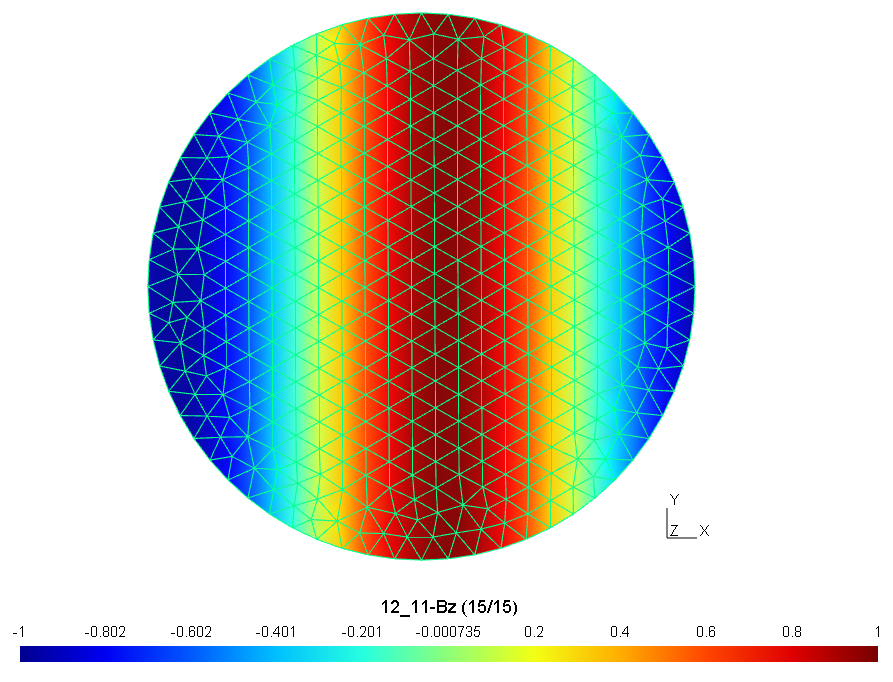
\includegraphics[height=7cm,keepaspectratio=true]{./fig/Fig1.png}
\caption{Onde plane sur un cercle unité}
\end{figure}
\end{frame}


\begin{frame}

  \begin{figure}[h]
    \centering
    \begin{tikzpicture}[scale=0.5]
      \begin{loglogaxis}[x=4cm,
        xlabel=$h$,ylabel=$\|\mathbf{W}^{ex}-\mathbf{W}_{h}\|_{L_2}$,
        legend style={at={(0,1.4)}, anchor=north west}]
        \addplot table[x=h,y={create col/linear regression={y=order1}}]{order1.dat};
        \xdef\slopea{\pgfplotstableregressiona}
        \addlegendentry{Ordre $d=1$ : $\log{erreur}$, pente = 0.94}
		 \addplot table[x=h,y={create col/linear regression={y=order2}}]{order2.dat};
        \xdef\slopea{\pgfplotstableregressiona}
        \addlegendentry{Ordre $d=2$ : $\log{erreur}$, pente =2.25}
		 \addplot table[x=h,y={create col/linear regression={y=order3}}]{order3.dat};
        \xdef\slopea{\pgfplotstableregressiona}
        \addlegendentry{Ordre $d=3$ : $\log{erreur}$, pente = 3.48}
		 \end{loglogaxis}
    \end{tikzpicture}
     \caption{Étude de la convergence spatiale, erreur entre la solution exacte et approchée en norme $L_2$ en fonction de $h$. $t=0.5s$, Composante $bz$}
    \label{fig:res}
  \end{figure}
\end{frame}




\begin{frame}
\frametitle{Résultats graphiques II}
\begin{figure}
\centering
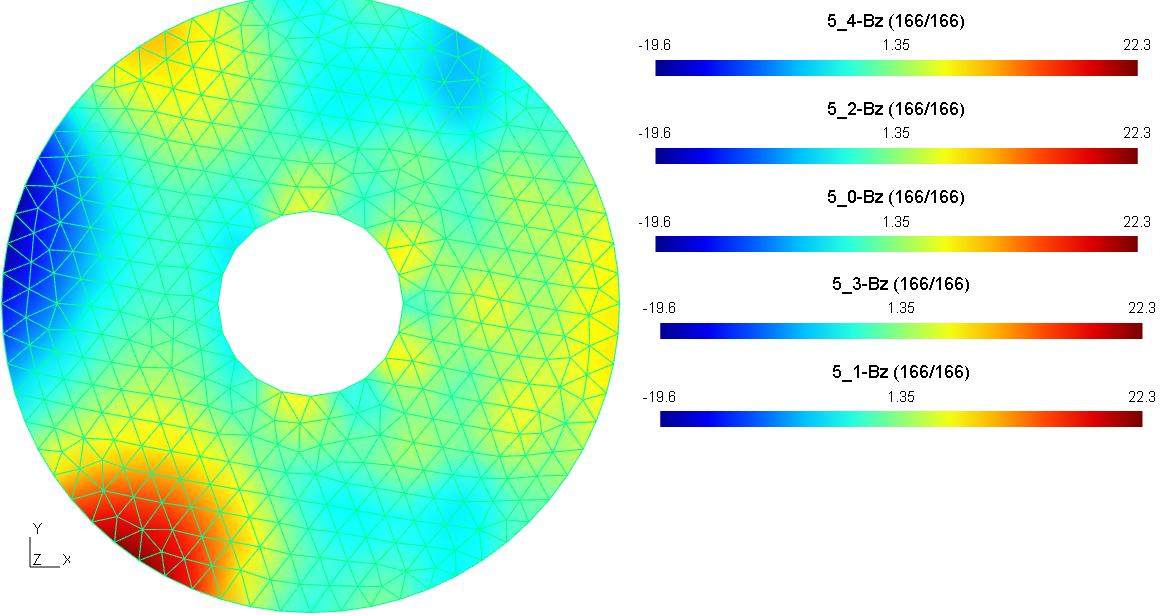
\includegraphics[height=6cm,keepaspectratio=true]{./fig/Fig2.png}
\caption{Onde plane sur un cercle unité percé. Condition métallique sur le cercle central $t=1$}
\end{figure}
\end{frame}




\begin{frame}
\frametitle{Un pas vers le 3D...}
Equations 3D Maxwell sans terme source, géométrie cartésienne,
\begin{eqnarray}
\partial_t E_x - \partial_y H_z + \partial_z H_y    &=& 0, \label{eq:3a}\\
\partial_t E_y - \partial_z H_x + \partial_x H_z    &=& 0, \label{eq:3b}\\
\partial_t E_z - \partial_x H_y + \partial_y H_x    &=& 0, \label{eq:3c}\\
\partial_t H_x + \partial_y E_z - \partial_z E_y    &=& 0, \label{eq:3d}\\
\partial_t H_y + \partial_z E_x - \partial_x E_z    &=& 0, \label{eq:3e}\\
\partial_t H_z + \partial_x E_y - \partial_y E_x    &=& 0, \label{eq:3f}.
\end{eqnarray}
\end{frame}





\begin{frame}
\frametitle{Un pas vers le 3D...}
En notant par $\mathbf{W}$ et $\mathbf{A}^1$, $\mathbf{A}^2$ les matrices tels que
\begin{equation}
\mathbf{W}=
\begin{pmatrix}
E_x\\
E_y\\
E_z\\
H_x\\
H_y\\
H_z\\
\end{pmatrix},
\qquad
\mathbf{A}^1=
\begin{pmatrix}
0 & 0 & 0 & 0 & 0 & 0\\
0 & 0 & 0 & 0 & 0 & 1\\
0 & 0 & 0 & 0 & -1 & 0\\
0 & 0 & 0 & 0 & 0 & 0\\
0 & 0 & -1 & 0 & 0 & 0\\
0 & 1 & 0 & 0 & 0 & 0\\
\end{pmatrix},
\end{equation}
\end{frame}


\begin{frame}
\frametitle{Un pas vers le 3D...}
\begin{equation}
\mathbf{A}^2=
\begin{pmatrix}
0 & 0 & 0 & 0 & 0 & -1\\
0 & 0 & 0 & 0 & 0 & 0\\
0 & 0 & 0 & 1 & 0 & 0\\
0 & 0 & 1 & 0 & 0 & 0\\
0 & 0 & 0 & 0 & 0 & 0\\
-1 & 0 & 0 & 0 & 0 & 0\\
\end{pmatrix},
\qquad
\mathbf{A}^3=
\begin{pmatrix}
0 & 0 & 0 & 0 & 1 & 0\\
0 & 0 & 0 & -1 & 0 & 0\\
0 & 0 & 0 & 0 & 0 & 0\\
0 & -1 & 0 & 0 & 0 & 0\\
1 & 0 & 0 & 0 & 0 & 0\\
0 & 0 & 0 & 0 & 0 & 0\\
\end{pmatrix}
\end{equation}
\end{frame}



\begin{frame}
\frametitle{Un pas vers le 3D...}

\begin{equation}
\mathbf{A}^in_i^+=
\begin{pmatrix}
\frac{{n2}^{2}+{n3}^{2}}{2\,r} & -\frac{n1\,n2}{2\,r} & -\frac{n1\,n3}{2\,r} & 0 & \frac{n3}{2} & -\frac{n2}{2}\cr
 -\frac{n1\,n2}{2\,r} & \frac{{n1}^{2}+{n3}^{2}}{2\,r} & -\frac{n2\,n3}{2\,r} & -\frac{n3}{2} & 0 & \frac{n1}{2}\cr
 -\frac{n1\,n3}{2\,r} & -\frac{n2\,n3}{2\,r} & \frac{{n2}^{2}+{n1}^{2}}{2\,r} & \frac{n2}{2} & -\frac{n1}{2} & 0\cr
 0 & -\frac{n3}{2} & \frac{n2}{2} & \frac{{n2}^{2}+{n3}^{2}}{2\,r} & -\frac{n1\,n2}{2\,r} & -\frac{n1\,n3}{2\,r}\cr
 \frac{n3}{2} & 0 & -\frac{n1}{2} & -\frac{n1\,n2}{2\,r} & \frac{{n1}^{2}+{n3}^{2}}{2\,r} & -\frac{n2\,n3}{2\,r}\cr
 -\frac{n2}{2} & \frac{n1}{2} & 0 & -\frac{n1\,n3}{2\,r} & -\frac{n2\,n3}{2\,r} & \frac{{n2}^{2}+{n1}^{2}}{2\,r}
 \end{pmatrix}
  \end{equation}
\end{frame}


\begin{frame}
\frametitle{Un pas vers le 3D...}
 \begin{equation}
 \mathbf{A}^in_i^-=
 \begin{pmatrix}
 -\frac{{n2}^{2}+{n3}^{2}}{2\,r} & \frac{n1\,n2}{2\,r} & \frac{n1\,n3}{2\,r} & 0 & \frac{n3}{2} & -\frac{n2}{2}\cr
 \frac{n1\,n2}{2\,r} & -\frac{{n1}^{2}+{n3}^{2}}{2\,r} & \frac{n2\,n3}{2\,r} & -\frac{n3}{2} & 0 & \frac{n1}{2}\cr 
 \frac{n1\,n3}{2\,r} & \frac{n2\,n3}{2\,r} & -\frac{{n2}^{2}+{n1}^{2}}{2\,r} & \frac{n2}{2} & -\frac{n1}{2} & 0\cr
 0 & -\frac{n3}{2} & \frac{n2}{2} & -\frac{{n2}^{2}+{n3}^{2}}{2\,r} & \frac{n1\,n2}{2\,r} & \frac{n1\,n3}{2\,r}\cr
 \frac{n3}{2} & 0 & -\frac{n1}{2} & \frac{n1\,n2}{2\,r} & -\frac{{n1}^{2}+{n3}^{2}}{2\,r} & \frac{n2\,n3}{2\,r}\cr
 -\frac{n2}{2} & \frac{n1}{2} & 0 & \frac{n1\,n3}{2\,r} & \frac{n2\,n3}{2\,r} & -\frac{{n2}^{2}+{n1}^{2}}{2\,r}
 \end{pmatrix}.
 \end{equation}
\end{frame}




\begin{frame}
\frametitle{Travaux futurs}
Au re-preneur de ce projet...
\begin{enumerate}
\item Trouver des containers appropriés pour le passage aux fonctions
\item Trouver la bonne macro pour Legendre
\item Créer une fonction solution exacte (code actuellement dupliqué)
\item Évaluation de l'ordre en temps, et de l'accumulation d'erreur degré faible
\item Interfacage avec les solveurs TS de \texttt{petsc}
\item Traitement du terme source
\item Ajout de la correction de la divergence
\item Etudes des conditions aux bords Benchmark 3D.
\end{enumerate}
\end{frame}









\begin{frame}
\frametitle{Retour sur l'expérience}
\begin{enumerate}
\item ++\quad Découvrir de manière plus approfondie la syntaxe \texttt{Feel++}
\item ++\quad Enrichir mes connaissances sur les systèmes hyperboliques linéaires ainsi que sur la méthode Galerkin Discontinue
\item -\, - \quad Manque crucial de temps.
\end{enumerate}
\end{frame}







% \begin{frame}
% \frametitle{Architecture serveur}
% \framesubtitle{Choix}
% \begin{figure}
% \centering
% \includegraphics[height=7.5cm,keepaspectratio=true]{./fig/archi2.png}
% \caption{Architecture serveur}
% \end{figure}
% \endframe}




% \begin{frame}
% \frametitle{Protocole applicatif (UDP) II}
 % \begin{figure}[!h]
% \begin{center}	
% \includegraphics[width=0.9\textwidth]{./fig/proto.png}
% \caption{\label{fig1}Datagramme UDP employé entre les CO et le serveur.} 
% \end{center}
% \end{figure}
 % \end{frame}

 
 
% \begin{frame}
% \vfill
% \begin{center}
% \Large Bilan
% \end{center}
% \vfill
% \end{frame}
 
 
 
 
\begin{frame}
\vfill
\begin{center}
\Large Merci
\end{center}
\vfill
\end{frame}



\end{document}
